%-------------------------------------------------------------------------------
\section{Problem}\label{s:problem}
%-------------------------------------------------------------------------------


\begin{figure}[t]
    \centering
    \begin{subfigure}[b]{0.49\columnwidth}
        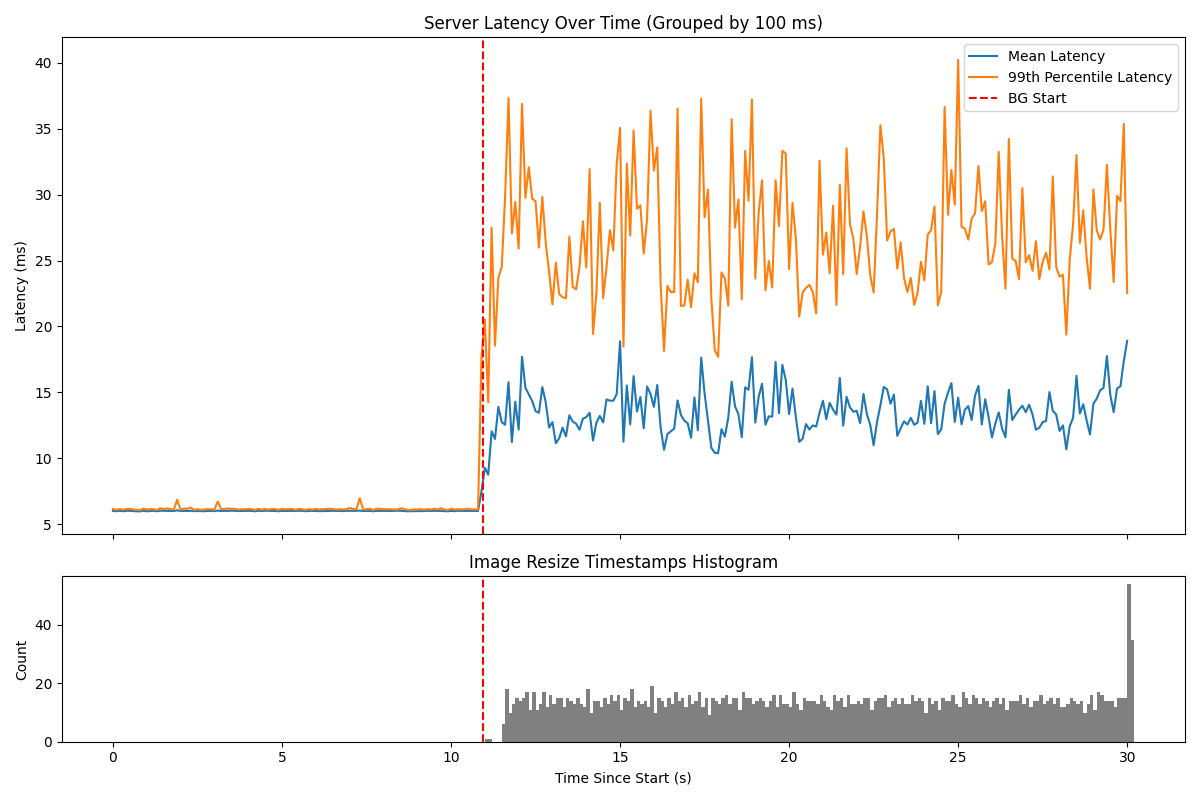
\includegraphics[width=\columnwidth]{graphs/srv-bg-unedited-low.png}
        \caption{Low load stetting, utilization before starting the BE tasks is
        around 85\%}\label{fig:srv-bg-unedited-low}
    \end{subfigure}
    \hspace{\fill}
    \begin{subfigure}[b]{0.49\columnwidth}
        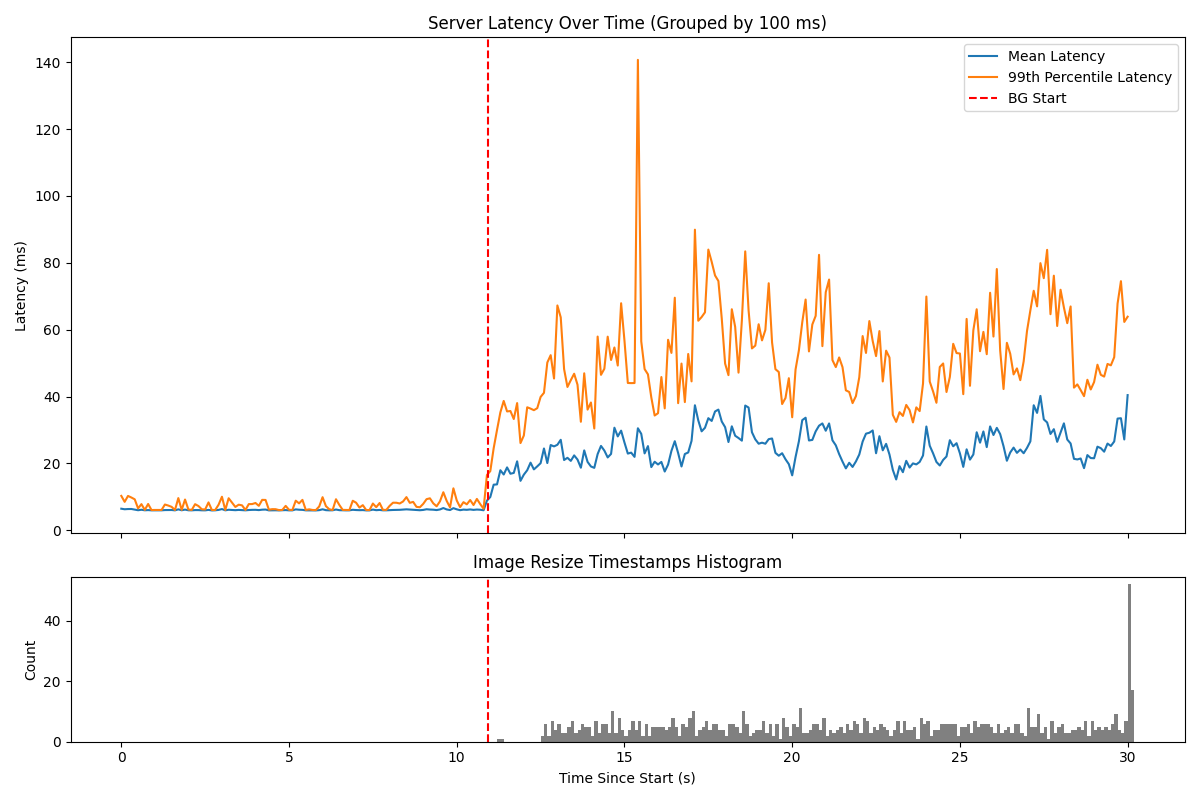
\includegraphics[width=\columnwidth]{graphs/srv-bg-unedited-high.png}
        \caption{High load setting, utilization before starting the BE tasks is
        around 95\%}\label{fig:srv-bg-unedited-high}
    \end{subfigure}
    \vspace{4pt}
    \caption{Latencies of the server and iteration counts of the background
    tasks in different load scenarios. Note the different y axis limits. The
    upper graphs show end-to-end request latencies, and the bottom graph is a
    histogram of completed iterations of the BE tasks}\label{fig:srv-bg-unedited}
\end{figure}

In order to understand more concretely where the isolation between the LC web
application and the BE image resize is failing in
\autoref{fig:kubernetes-unedited}, we reproduce the jump in latency we saw in
the application running on Kubernetes in a simpler benchmark. We run a simple
cpu-bound server with a pool of worker threads that we hit with an open-loop
remote client, and then start two BE workloads doing image resizing. We put the
LC server and the BE resize job each in their own \cgroups{} group, with weights
1 and 10000. \autoref{fig:srv-bg-unedited} shows the increase in latencies of
the LC server at two different baseline utilization levels. We see that even in
the lower baseline utilization case, where the server alone uses 85\%, mean
latencies spike up from steady at around 6ms to as high as 20ms, and much higher
for 99th percentile latencies.

\begin{figure}[t]
    \centering
    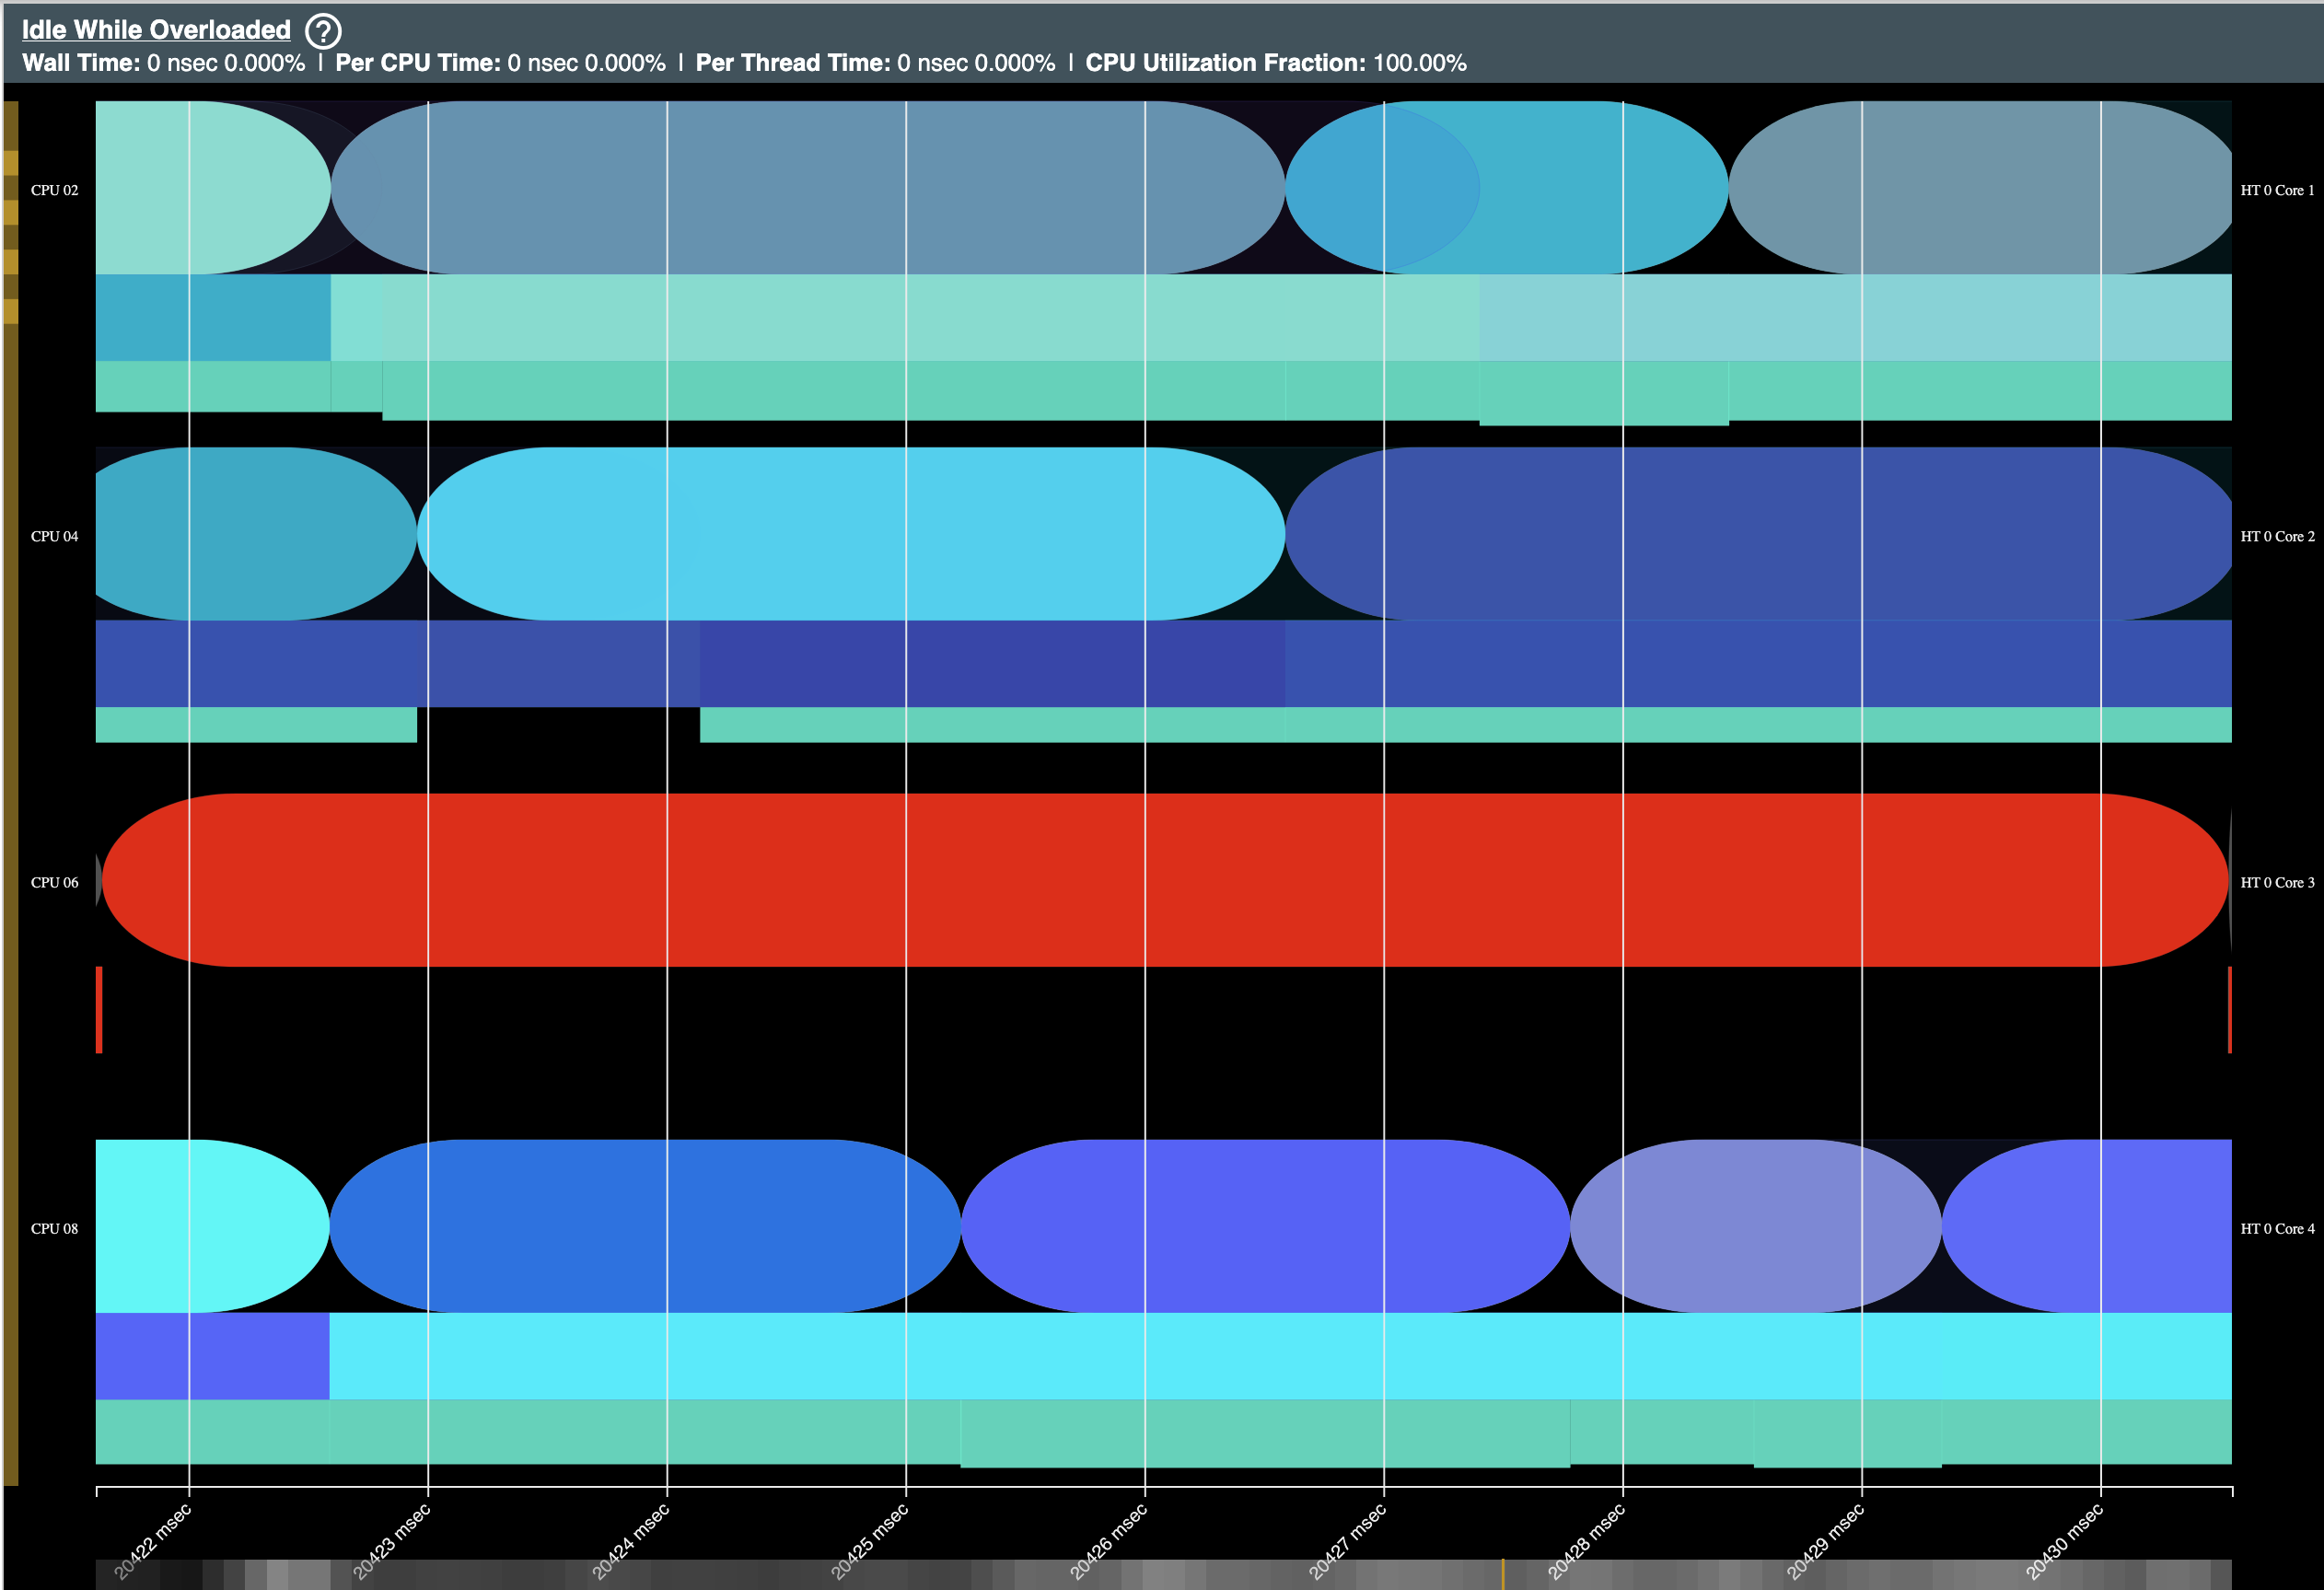
\includegraphics[width=\columnwidth]{graphs/schedviz-problem.png}
    \caption{Each thread is a different color. Circles represent which
    thread is running on that core, while rectangles underneath show waiting but
    runnable threads
    }\label{fig:schedviz-problem}
\end{figure}

Using this simplified experiment, we analyze perf traces of the scheduling
decisions, and visualize the trace using schedviz~\cite{schedviz-tool}, in order
to understand where the latency impact comes from.
\autoref{fig:schedviz-problem} shows a 10ms outtake of the resulting image. The
process running on each core is shown as a an oval, and queued processes are
shown as rectangles below. The root of the undesirable behavior is: on core 6,
the red process that is running the whole time is a BE process, whereas LC
threads, shown in varying shades of blue, are queued on the other cores. The
takeaway here is that the failure mode we observe is that \textit{one core is
running a BE process, while an LC process is waiting on another}.

Based on this observation, we explore more deeply the root of the issue that is
causing the poor behavior we see.

\subsection{Weights are only enforced locally}\label{ss:problem:mechanistic}

The reason this happens is that Linux maintains a separate runqueue on each
core, in order to avoid the synchronization overheads of accessing global state
for every scheduling decision. Within each runqueue, Linux's scheduler works to
maintain the correct ratio of received CPU time at each scheduling; but Linux
does not enforce the weight ratios across cores. This leads to the above failure
mode, where one core has no runnable high weight processes and thus runs a low
weight one, whereas another core has queued high weight processes. This problem
goes away when there are no BE processes, because cores try to steal work before
going idle.

\subsection{Enforcing weights across cores is
expensive}\label{ss:problem:cross-core-hard}

The root of the problem goes deeper than just a poor implementation: a
weight-based interface is at odds with machine-wide policy enforcement. In order
to strictly and globally enforce a processes weight, the scheduler would need to
synchronize at every scheduling decision: calculating whether a given process is
owed time globally requires knowing the total weight across all cores as well as
the sum of time that all the processes in the group have gotten. In increasingly
multi-core and multi-NUMA machines, synchronization is expensive; other work has
found that kernel lock contention is a bottleneck to performance at
scale.~\cite{afaas} This means that the overheads of maintaining global
invariants can quickly become prohibitive.


\subsection{Weights interact poorly with tick-based
scheduling}\label{ss:problem:quantum}

Even on a single runqueue, using very large weight differentials as an interface
to isolate LC and BE doesn't work well because preemption is tick-based. In a
weight based scheme, BE processes also get a fair share of the CPU. The problem
is that, when this happens, the BE process will interrupt any running LC process
for a whole tick. In Linux, hardware ticks are 4ms long. This means that an LC
thread processing a request may be interrupted for up to 4ms, provided the BE
process runs for that long before blocking. 4ms can be a large amount of time
for microservice workloads, whose SLOs are often in the low double digit or even
single digit ms realm.~\cite{sigmaos}



